\section{Related Work}
\label{sec:formatting}

\begin{figure*}
\begin{minipage}[t]{0.52\linewidth}
    \centering
    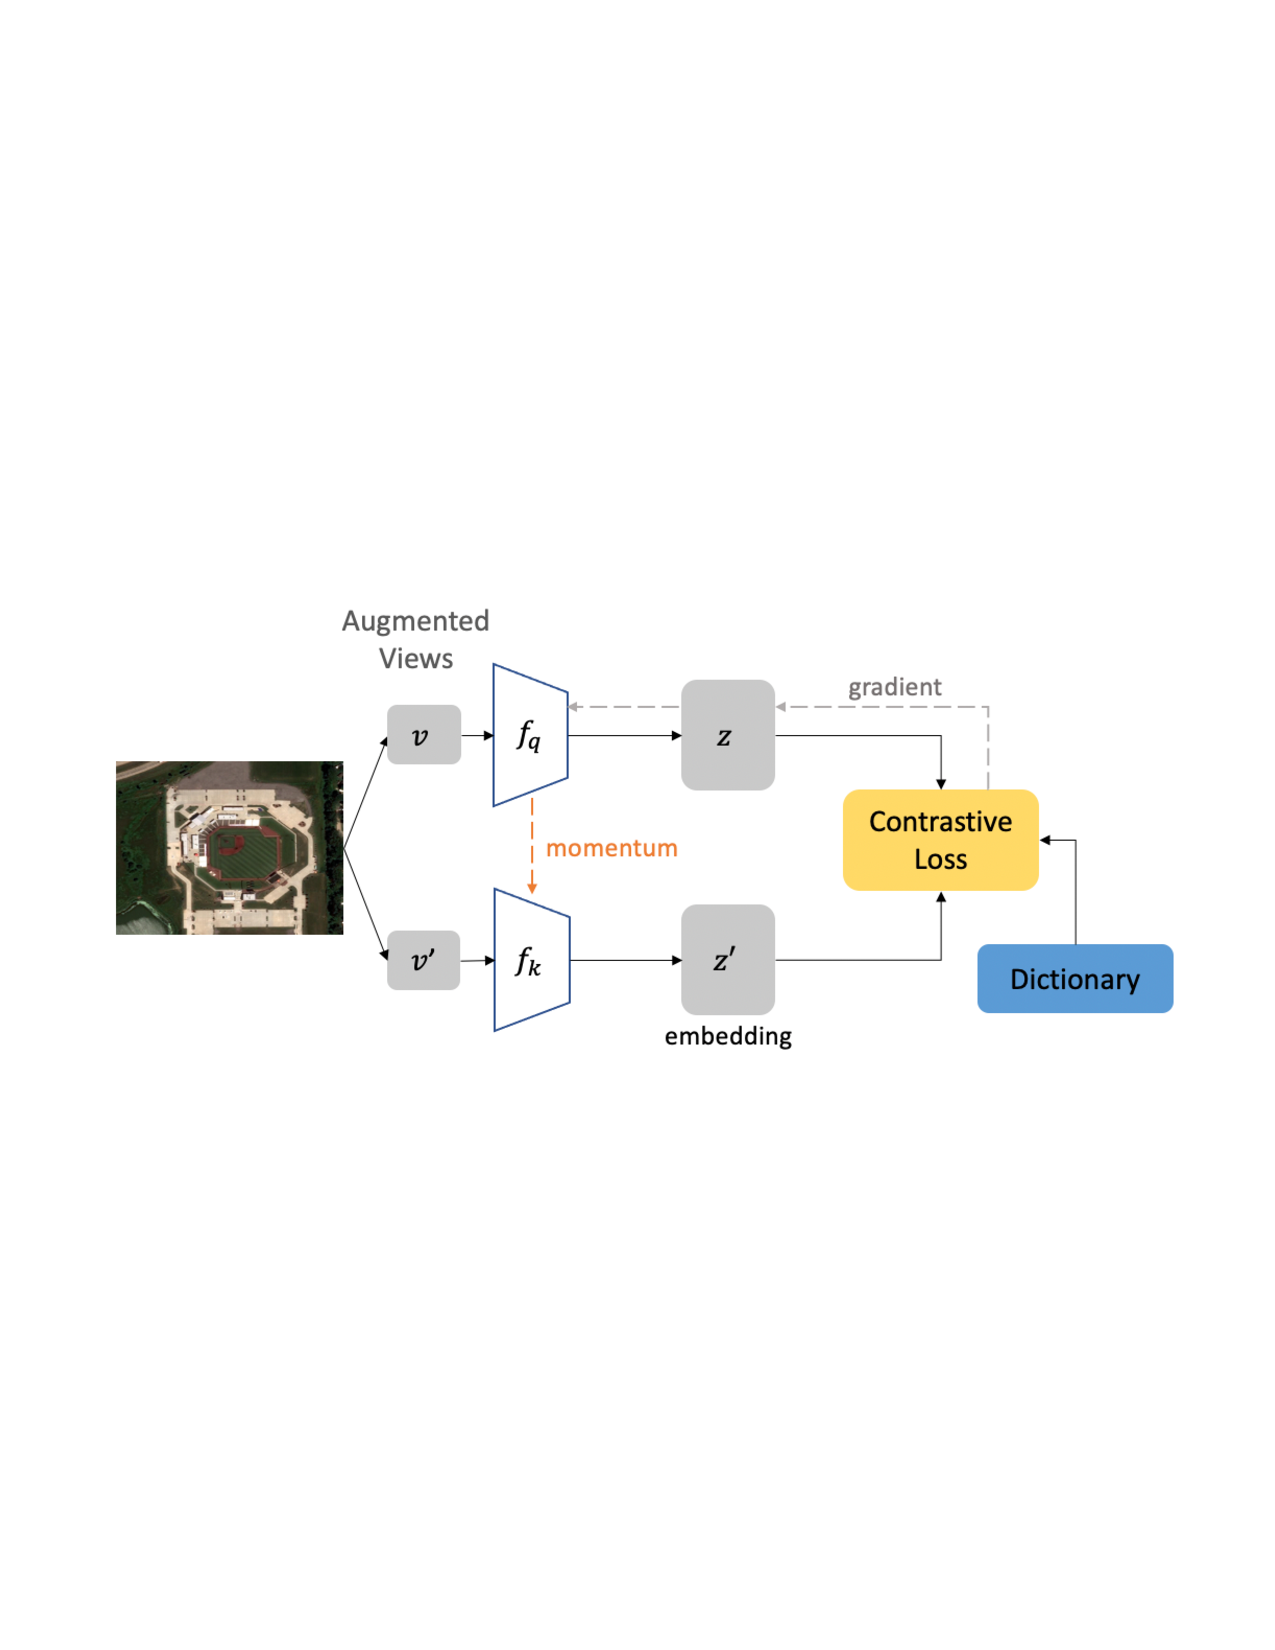
\includegraphics[width=\linewidth]{figures/ap1.pdf}
    \caption{Schematic overview of the original MoCo-v2 framework \\(figure by \cite{geoAwareSelfSuper}).}
    \label{fig:Moco}
\end{minipage}
\hfill
\begin{minipage}[t]{0.44\linewidth}
    \centering
    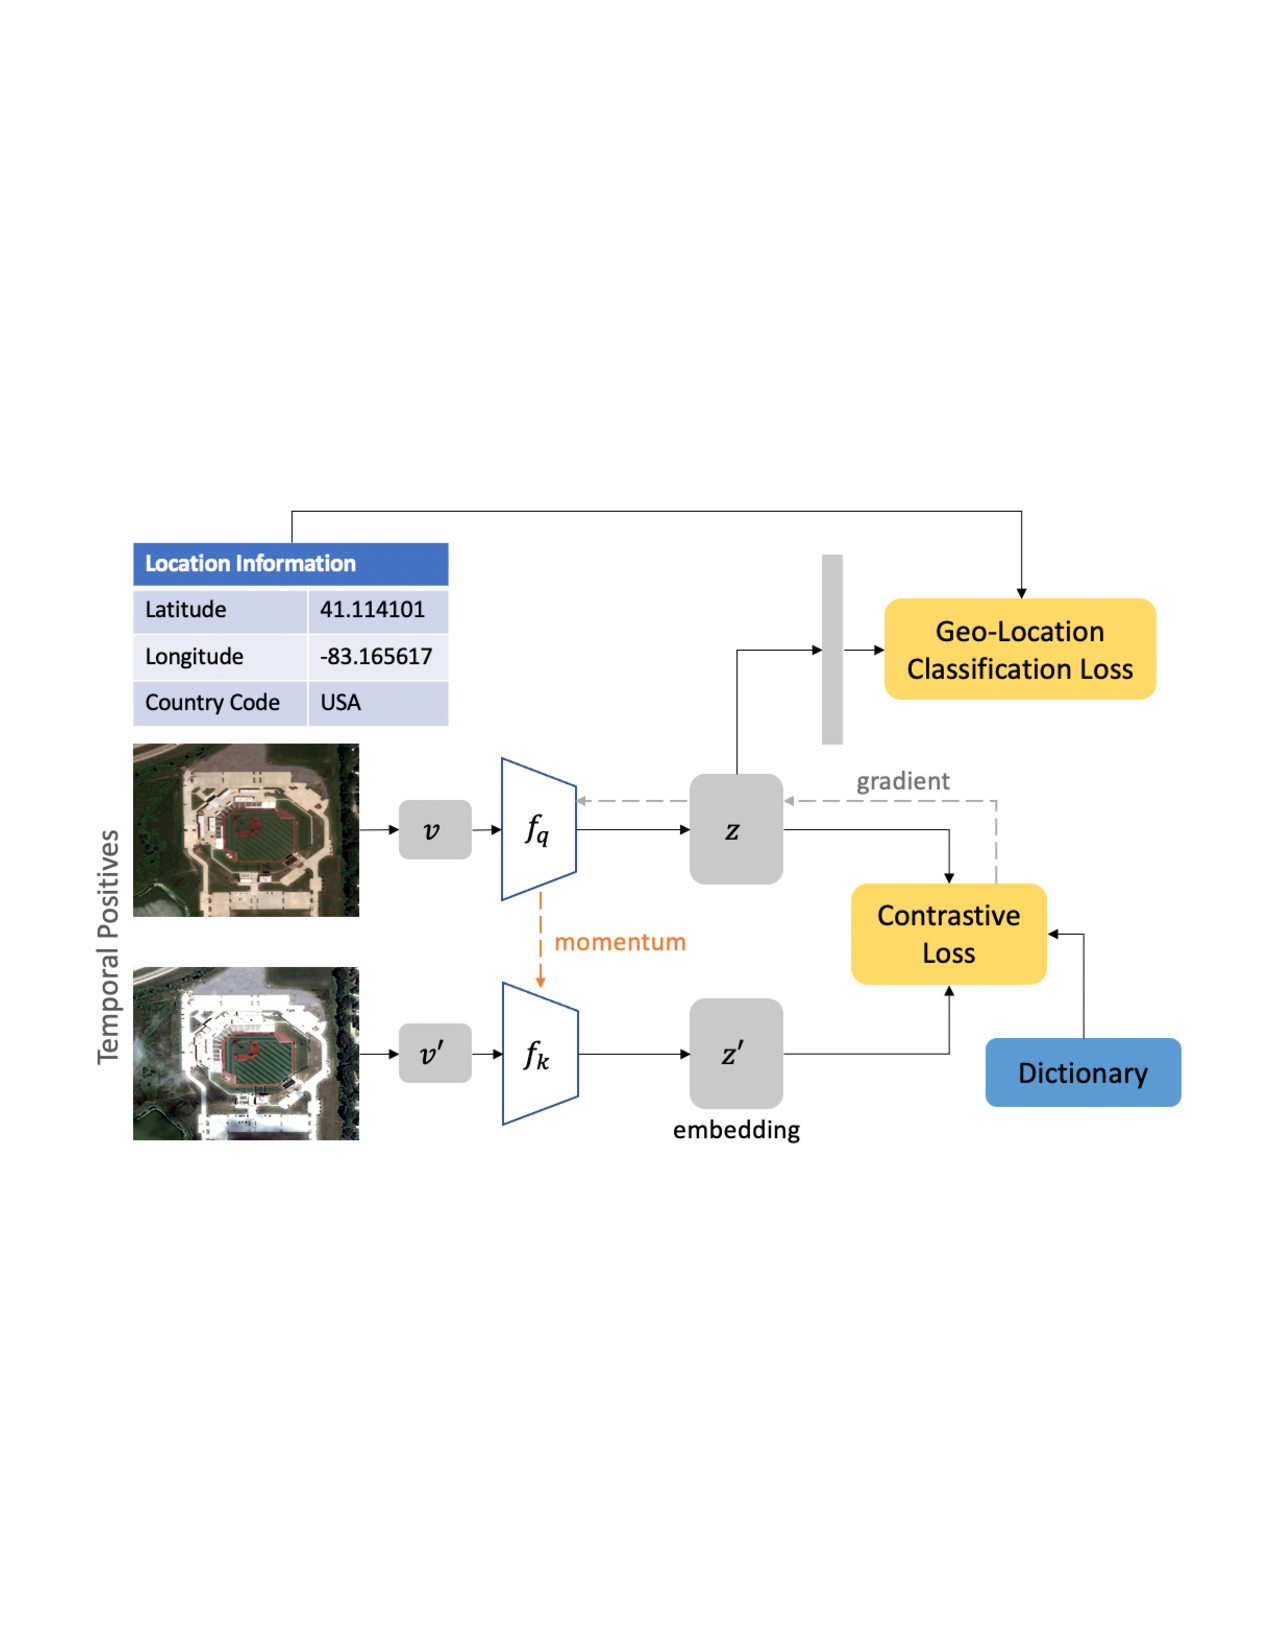
\includegraphics[width=\linewidth]{figures/ap2.pdf}
    \caption{Geography-aware contrastive learning approach (figure by \cite{geoAwareSelfSuper}).}
    \label{fig:geography_aware}
\end{minipage}
\end{figure*}

Self-supervised models for satellite data face several challenges due to the unique characteristics of the data, such as the temporal dimension, their large-scale nature and the availability of data from various complementary sensors \cite{presto}. These factors complicate the modeling process, requiring the use of sophisticated foundation model techniques. \\
Most state-of-the-art models are based on transformer networks, often in combination with masked autoencoders. Transformer models are designed to handle sequential data, weighing the importance of different elements within the sequence \cite{transformer}. This capability makes them particularly well-suited for the temporal dimension of satellite data, where capturing long-range dependencies and relationships is crucial. \\
In a masked autoencoder parts of the input data are hidden during training, and the model learns to reconstruct the missing parts from the remaining visible parts \cite{maskedAutoEncoder}. This approach is particularly useful for learning robust feature representations and dealing with incomplete data. Masked autoencoders benefit from the powerful feature extraction capabilities of transformers. By using a transformer as the backbone, the model can effectively handle sequential and high-dimensional data. Examples are SatMAE \cite{SatMAE}, Presto \cite{presto} and RVSA \cite{rvsa}. These models use techniques like temporal embeddings, masking image patches across time and associated metadata. RVSA introduces a lage-scale vision transformer which replaces the full attention in transformers with a new rotated varied-size window attention to reduce computational cost and memory footprint. \\
Other approaches train diffusion models like DiffusionSat \cite{DiffSat} and PreDiff  \cite{prediff}. A diffusion model is a type of generative model that gradually transforms noise into a target data distribution through a series of iterative steps, often used for data generation \cite{diffusion}. DiffusionSat conditions the model on metadata such as geolocation to generate realistic samples, while PreDiff introduces a two-stage pipeline for probabilistic spatiotemporal forecasting. \\
There are other self-supervised learning methods used in foundation models for Earth observation that have received less attention in the literature. One such method is contrastive learning which trains models by distinguishing between similar (positive pairs) and dissimilar data pairs. This approach encourages closeness of representations of images that are likely to be semantically similar. \cite{geoAwareSelfSuper} \\
In this paper the quality of the contrastive learning foundation models introduced by K. Ayush et al. \cite{geoAwareSelfSuper} are exaulated on a remote sensing dataset.

